\scanpage{107}
% archive foliation: 106 (first digit partly clipped)
\figure{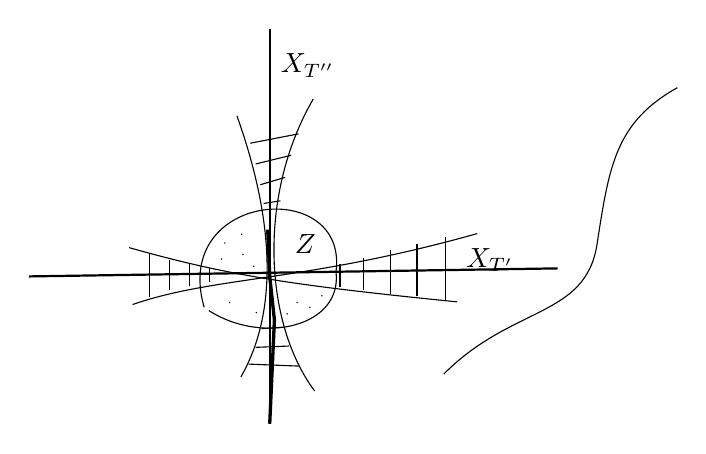
\begin{tikzpicture}[x=0.85cm,y=0.85cm]
\draw[thick] (-3.6,0)--(4.3,0.12);
\draw[thick] (0,-2.2)--(0,3.7);
\draw[very thick] (0,-2.2)--(0.07,-0.65)--(0,0)--(-0.03,0.7);
\draw (-2.1,0.43) .. controls (-0.65,0.02) and (0.3,-0.13) .. (2.8,-0.38);
\draw (-2.05,-0.42) .. controls (-0.8,0.01) and (0.5,-0.09) .. (3.1,0.64);
\draw (-0.49,2.40) .. controls (0.08,0.80) and (0.12,-0.54) .. (-0.43,-1.50);
\draw (0.65,2.65) .. controls (-0.18,1.22) and (-0.09,-0.69) .. (0.67,-1.71);
\draw (-0.29,1.99)--(0.43,2.13);
\draw (-0.21,1.68)--(0.32,1.81);
\draw (-0.14,1.37)--(0.23,1.48);
\draw (-0.09,1.09)--(0.16,1.13);
\draw (-0.12,-0.78)--(0.18,-0.76);
\draw (-0.21,-1.06)--(0.29,-1.04);
\draw (-0.32,-1.31)--(0.44,-1.34);
\foreach \x/\lo/\hi in {-1.8/-0.31/0.34,-1.5/-0.21/0.25,-1.2/-0.15/0.18,-0.9/-0.09/0.12,1.05/-0.16/0.18,1.4/-0.20/0.28,1.8/-0.26/0.39,2.2/-0.30/0.49,2.62/-0.36/0.59}{\draw (\x,\lo)--(\x,\hi);}
\draw (-0.98,-0.46) .. controls (-1.48,1.28) and (1.18,1.49) .. (0.99,0.07)
 .. controls (1.09,-0.75) and (-0.10,-1.03) .. (-0.91,-0.51);
\foreach \x/\y in {-0.67/0.50,-0.42/0.63,-0.72/0.26,-0.40/0.33,-0.24/0.15,-0.60/-0.39,-0.20/-0.54,0.26/-0.56,0.41/-0.39,0.60/-0.46,0.78/-0.29,0.54/0.62}{\fill (\x,\y) circle (0.012);}
\node at (0.53,0.48) {$Z$};
\node at (3.29,0.24) {$X_{T'}$};
\node[right] at (0.02,3.15) {$X_{T''}$};
\draw (2.6,-1.46) .. controls (3.62,-0.43) and (4.72,-0.62) .. (4.89,0.48)
 .. controls (5.07,1.64) and (5.16,2.30) .. (6.09,2.82);
\end{tikzpicture}}

\margin{$*$}
\diagram{\begin{tikzcd}[column sep=small,row sep=large]
\widehat{\mathbf Z}=\unsure{\Pi|\pi}_1(Z') \arrow[d] \arrow[drr] & & \unsure{\Pi|\pi}_1(Z'')=\widehat{\mathbf Z} \arrow[dl] \arrow[d] \\
\unsure{\Pi|\pi}_1(X_{T'}) \arrow[dr] & \unsure{\Pi|\pi}_1(X_{T''}) \arrow[d] & \unsure{\Pi|\pi}_1(Z)=\widehat{\mathbf Z}^{2} \arrow[dl] \\
& \unsure{\Pi|\pi}_1(X_T) &
\end{tikzcd}}

\figure{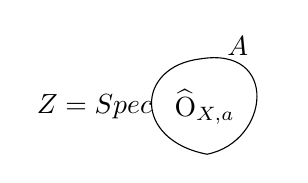
\begin{tikzpicture}
\node at (-1.4,0) {$Z=\operatorname{Spec}$};
\node at (0,0) {$\widehat{\mathrm O}_{X,a}$};
\draw (0.03,-0.60) .. controls (-0.91,-0.42) and (-0.88,0.51) .. (-0.06,0.61)
 .. controls (0.95,0.78) and (0.83,-0.44) .. (0.03,-0.60);
\node at (0.42,0.77) {$A$};
\end{tikzpicture}}
\[
X_{T'}\cap X_{T''}=\varnothing
\]
\[
X_{T'}\cap Z_{\deleted{\unsure{a}}}=Z'=\widehat A_{\unsure{p'|\mathfrak p'}}
\quad\begin{gathered}\unsure{correspond} -- \text{corps}\\
\text{résiduel }k(p')=\text{corps local en }a\text{ de }T'_0
\end{gathered}
\]
\[
X_{T''}\cap Z=Z''=\widehat A_{\unsure{p''|\mathfrak p''}}
\quad\begin{gathered}\unsure{correspond} -- \text{corps}\\
\text{résiduel }k(p'')=\text{corps local en }a\text{ de }T''_0
\end{gathered}
\]

On doit prouver un \uline{\unsure{th.} de descente} de nature essentiellement locale

$+$ déterminer certains \unsure{hom.} canoniques

\figure{\begin{tikzpicture}\draw (0,0)--(0.2,0.04);\draw (0.4,0.02)--(1.25,0.03);\draw (1.55,0.04)--(2.15,0.04);\end{tikzpicture}}

\margin{\diagram{\begin{tikzcd}[row sep=small]
\deleted{\unsure{A'}}\unsure{\}} \arrow[d,dash,bend right=30] \\
A \arrow[d] \\
B
\end{tikzcd}}}
